\documentclass[xcolor=dvipsnames]{beamer}
\usefonttheme{professionalfonts}
\usepackage{fontspec}
\setmainfont[BoldFont={RedHatDisplay-SemiBold.ttf}]{RedHatDisplay-Regular.ttf}
\setsansfont[BoldFont={RedHatDisplay-SemiBold.ttf}]{RedHatDisplay-Regular.ttf}
\setmonofont{RedHatDisplay-Light.ttf}
\usetheme{Madrid}
\useoutertheme[subsection=false]{miniframes}
\useinnertheme{circles}

\definecolor{UBCblue}{rgb}{0.93, 0.0, 0.0} % UBC Blue (primary)
\definecolor{UBCgrey}{rgb}{0.93, 0.0, 0.0} % UBC Grey (secondary)
\setbeamercolor{frametitle}{fg=UBCblue,bg=white}


\setbeamercolor{palette primary}{bg=UBCblue,fg=white}
\setbeamercolor{palette secondary}{bg=UBCblue,fg=white}
\setbeamercolor{palette tertiary}{bg=UBCblue,fg=white}
\setbeamercolor{palette quaternary}{bg=UBCblue,fg=white}
\setbeamercolor{structure}{fg=UBCblue} % itemize, enumerate, etc
\setbeamercolor{section in toc}{fg=UBCblue} % TOC sections

% Override palette coloring with secondary
\setbeamercolor{subsection in head/foot}{bg=UBCgrey,fg=white}
\setbeamertemplate{title page}[default][colsep=-4bp,rounded=true]

\title[Prometheus: Querying basics]{Prometheus: Querying basics}
\date{\today}
\author[Jakub Guzik]
{DPTP Knowledge Talk}
%\institute[Ra]{RamblingAcademic.com\\Nuts and Bolts of Research. Plus Some Rambling.}
\newcommand{\mli}[1]{\mathit{#1}}

\begin{document}
\logo{

\includegraphics[width=2.5cm]{redhat.png}
}
	\begin{frame}
		\titlepage
	\end{frame}

	\begin{frame}
		\tableofcontents
	\end{frame}

	\section{Data types}


	\begin{frame}
	\frametitle{Expression language data types}
		\begin{enumerate}
			\item Scalar - a simple numeric floating point value
\item String - a simple string value; currently unused
\item Instant vector
\item Range vector
		\end{enumerate}
	\end{frame}
	\begin{frame}
	\frametitle{Instant vector}
A set of time series containing a single sample for each time series, all sharing the same timestamp.

\[
\mli{CPU} _ \mli{load}=
\begin{bmatrix}
    \textcolor{blue}{\mli{CPU}_1}      \\
    \textcolor{green}{\mli{CPU}_2}   \\
    \textcolor{red}{\mli{CPU}_3}   \\
    \textcolor{brown}{\mli{CPU}_4}
\end{bmatrix}
=
\begin{bmatrix}
    \textcolor{blue}{9.99}      \\
    \textcolor{green}{12.13}   \\
    \textcolor{red}{14.31}   \\
    \textcolor{brown}{4.22}

\end{bmatrix} _{\mli{for\: T_{\mli{now}}}}
\]

\end{frame}

\begin{frame}
\frametitle{Range vector}
A set of time series containing a range of data points over time for each time series.
\[
\mli{CPU} _ \mli{load}=
\begin{bmatrix}
    \textcolor{blue}{4.23}      \\
    \textcolor{blue}{6.44}   \\
    \textcolor{blue}{12.32}   \\
    \textcolor{blue}{11.23}
\end{bmatrix}_\mli{CPU_1}
\begin{bmatrix}
    \textcolor{green}{3.13}      \\
    \textcolor{green}{5.74}   \\
    \textcolor{green}{11.92}   \\
    \textcolor{green}{2.43} \\
        \textcolor{green}{32.43} \\
\end{bmatrix}_\mli{CPU_2}
\begin{bmatrix}
    \textcolor{red}{4.99}      \\
    \textcolor{red}{21.14}   \\
    \textcolor{red}{1.12}   \\
\end{bmatrix}_\mli{CPU_3}
\begin{bmatrix}
    \textcolor{brown}{5.15}      \\
    \textcolor{brown}{19.24}   \\
    \textcolor{brown}{9.42}   \\
    \textcolor{brown}{21.87}
\end{bmatrix}_\mli{CPU_4}
\]

\footnotesize \centering For the time range of last 5 minutes.
\end{frame}

\begin{frame}
 \frametitle{Instant vectors and range vectors}
 \centering
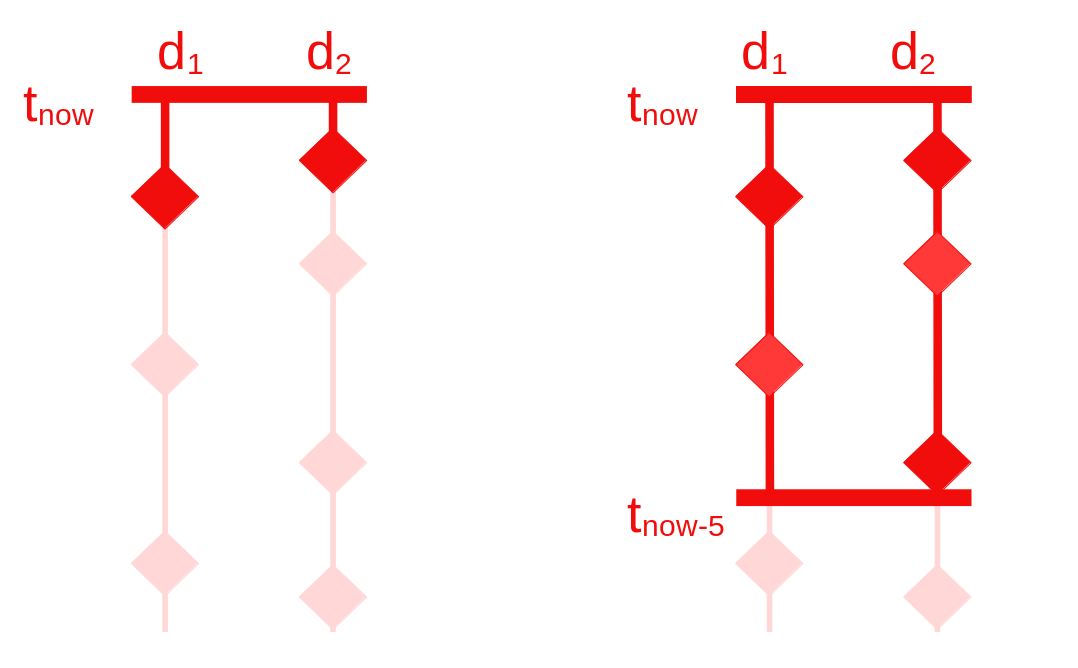
\includegraphics[width=0.65\textwidth]{vect.png}

Instant vector guarantees at least one value per time series while range vector guarantees any number of values between two timestamps.
\end{frame}
\section{Metric types}
\begin{frame}
 \frametitle{Available metrics}
 \begin{enumerate}
  \item Counter
  \item Gague
  \item Histogram
  \item Summary
 \end{enumerate}
\end{frame}
\begin{frame}
 \frametitle{Counter}
 \begin{itemize}
  \item  monotonically increasing counter
  \item value can reset on restart
 \end{itemize}
 \centering
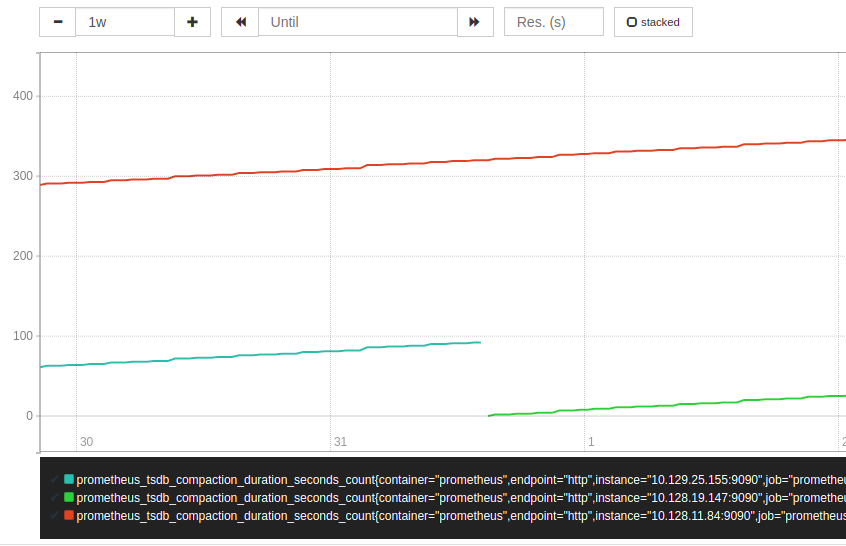
\includegraphics[width=0.65\textwidth]{counter.png}
\end{frame}

\begin{frame}
 \frametitle{Gague}
 \begin{itemize}
  \item  a metric that represents a single numerical value that can arbitrarily go up and down
  \item used for temperature, load, memory usage, concurrent requests
 \end{itemize}
 \centering
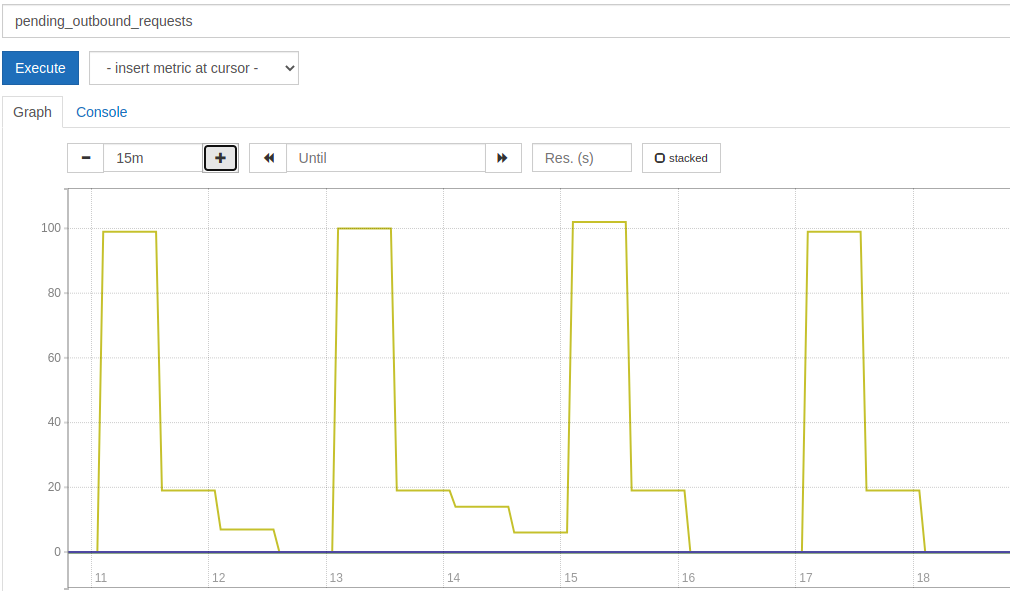
\includegraphics[width=0.65\textwidth]{gague.png}
\end{frame}

\begin{frame}
 \frametitle{Histogram \& Summary}
Histogram can be used for any calculated value which is counted based on bucket values. Bucket boundaries can be configured by the developer.
\begin{figure}
\centering
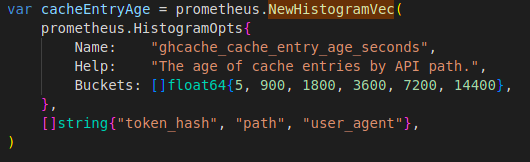
\includegraphics[width=0.65\textwidth]{code.png}

\end{figure}


Summary measures events and are an alternative to histograms.  It is used when the buckets of a metric is not known beforehand, but it is highly recommended to use histogram over summary whenever possible.

\end{frame}


\section{Operators}
\begin{frame}
 \frametitle{Binary operators}
Binary operators:
\begin{itemize}
\item arithmetic: +, -, /...
\item comparison: !=, ==, <...
\item set: and, or, unless
\end{itemize}
Binary operators accept scalars and instant vectors. \textbf{Labeling must be correct when using them with instatnt vectors.}
Aggregation operators:
\end{frame}

\begin{frame}
\frametitle{Aggregation operators}
\begin{itemize}
\item \texttt{sum()} calculate sum over dimensions
\item \texttt{min()} select minimum over dimensions
\item \texttt{max()} select maximum over dimensions
\item \texttt{avg()} calculate the average over dimensions
\item \texttt{count()} count number of elements in the vector
\item ...
\end{itemize}
Aggregation operators take an instant vector as input and output also an instant vector.
\end{frame}
\section{Functions/queries}
\begin{frame}
 \frametitle{Functions}
 Functions take an instant vector or a range vector as an input. The result always will be an instant vector.
\end{frame}
\begin{frame}
 \frametitle{\texttt{rate()}}
 \begin{itemize}
  \item Input: range vector
  \item Output: instant vector
  \item Description: calculates the per-second average rate of increase in the counter
 \end{itemize}
\vspace{0.2cm}
\begin{minipage}[t]{0.98\linewidth}
 \centering
 \texttt{rate(http\_requests\_total[5m])}
\end{minipage}
\vspace{0.8cm}

\texttt{rate()} function is special as breaks in monotonicity (like counter resets) are automatically adjusted for.

\vspace{0.4cm}
\texttt{rate()}, \texttt{increase()} and \texttt{irate()} are dedicated to use only with counters.
\end{frame}
\begin{frame}

 \frametitle{Demo}
 \centering
 \Huge \textbf{Demo!}

\end{frame}
\begin{frame}

 \frametitle{Sources}
\begin{itemize}
 \item \href{https://prometheus.io/docs/introduction/overview/}{Prometheus documentation}
 \item \href{https://www.robustperception.io/}{robustperception Blog}
 \item \href{https://www.youtube.com/watch?v=hTjHuoWxsks}{PromCon EU 2019: PromQL for Mere Mortals}
 \item \href{https://www.youtube.com/watch?v=hvACEDjHQZE}{How to build a PromQL (Prometheus Query Language)}
\end{itemize}


\end{frame}

\end{document}
